%! Author = Patrik Skaloš


% Preamble
\documentclass[a4paper]{article}


% Packages
\usepackage[utf8]{inputenc}
\usepackage[english]{babel}
\usepackage[T1]{fontenc}
\usepackage{geometry}
% \usepackage{amsmath, amssymb, amsthm}
\usepackage[unicode]{hyperref}
\usepackage{graphicx}

\usepackage{enumitem}

\newlist{notes}{enumerate}{1}
\setlist[notes]{label=Note: , leftmargin=2cm}

% Document
\begin{document}


  % Title page
  \begin{titlepage}

    \begin{center}

      \vspace*{5cm}

      \huge
      \textbf{A simple packet sniffer}
      
      \vspace{2cm}

      \huge
      \textbf{Patrik Skaloš}

      \vfill

      2022

    \end{center}

  \end{titlepage}


  % Table of contents
  \tableofcontents

  \newpage

  \section{Introduction}

  \subsection{Packet sniffing}

  Packet sniffing is an act of capturing frames that are being sent from or 
  received by a device on a certain network. Our program is able to capture 
  \textit{ethernet frames} on a single interface specified by the user.
  After a frame has been captured, various information about it can be printed, 
  including source and destination addresses, ports and even the encapsulated 
  data (although it is often encrypted).

  \subsection{Protocols}

  \textit{Protocols} will be mentioned many times in this document, but what 
  are they? They are simply sets of standards (rules) by which, for example, 
  data is encapsulated, transferred and so on. Without protocols, networking 
  would be a total chaos and thanks to them, it is very simple for devices to 
  read any data received since they can rely on those rules.


  \subsubsection{OSI model}
  
  To explain the protocols supported by our packet sniffer, we must first 
  introduce the OSI conceptual model of a networking system. Everything 
  important to understand can be explained by figure 1.

  % TODO cite https://techsoftcenter.com/osi-model/

  \begin{figure}[h]
    \centering
    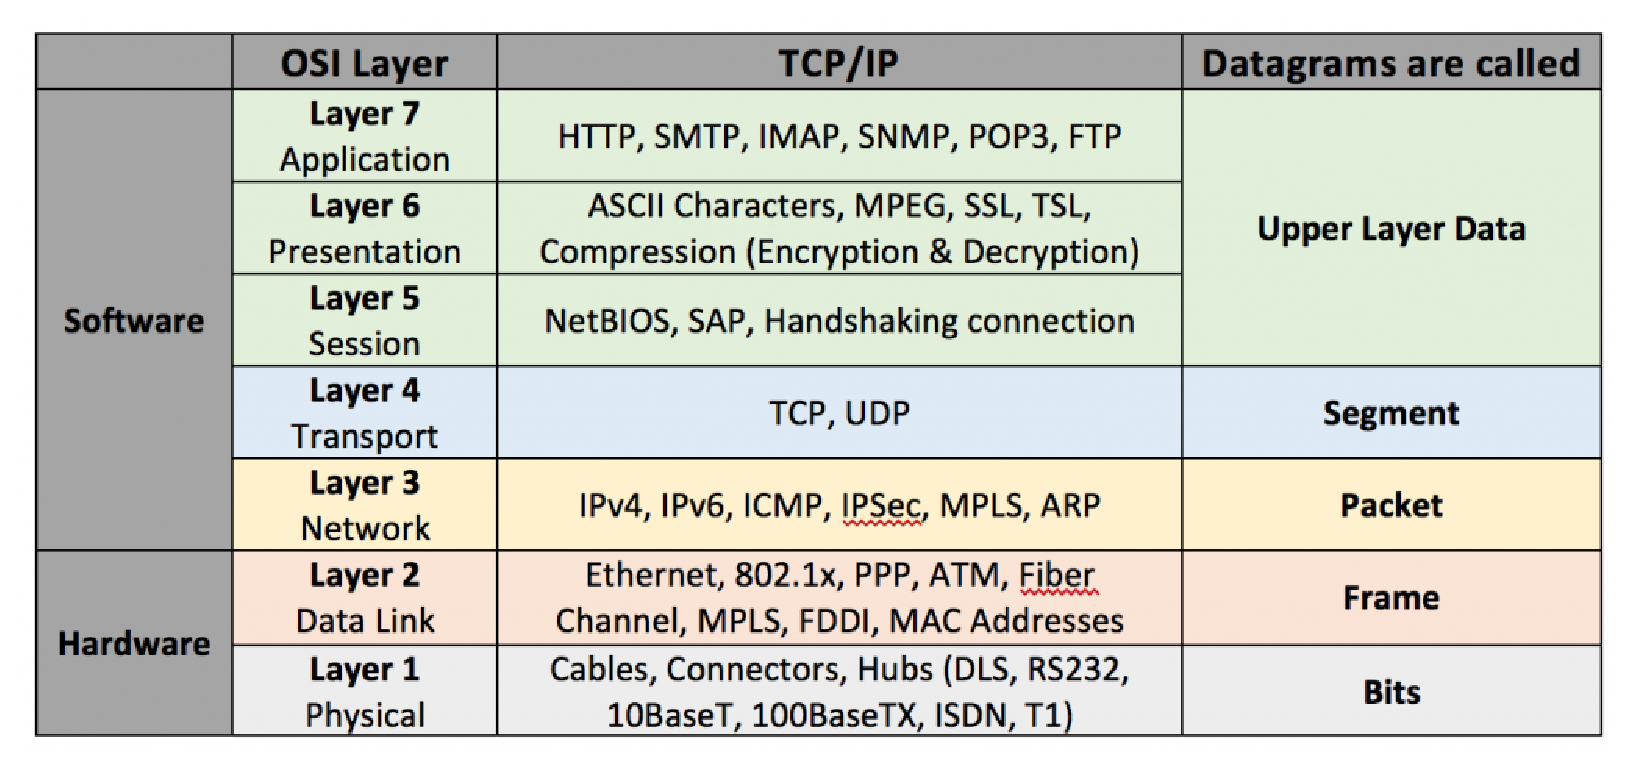
\includegraphics[width=\textwidth]{./src/osi.eps}
    \caption{OSI model}
  \end{figure}

  \subsubsection{Data units}

  Before any data can be sent over a network, it has to be formatted according
  to rules that various protocols provide. We need to understand differences
  between these data units:
  \begin{itemize}
    \item Frame: encapsulates a packet
    \item Packet: encapsulates a data segment
    \item Segment: encapsulates data
  \end{itemize}
  So, for example, sending a HTTP request from the application layer means
  dividing it into several portions if it is too big, encapsulating each portion
  to a segment, then to a packet and finally to a frame before representing the 
  frame as bits and sending it over a network media (e.g. cable).

  \begin{notes}
    \item Encapsulation means taking some data and adding metadata to it (in
      networking, metadata consists of a header and sometimes a trailer).
    \item It might be a bit confusing that a packet sniffer captures frames and
      not packets. I don't feel confident exaplaining why, but according to my
      research, word \textit{packet} is often used when referring to frames or 
      even segments and yes, to be precise, it should be called 
      \textit{frame sniffer} instead of \textit{packet sniffer}.
  \end{notes}

  \vspace{1cm}


  \subsection{Supported protocols}

  \subsubsection{Data link layer protocols}

  \textbf{Ethernet frame} is a data link layer protocol data unit in 
  which a packet is encapsulated along with MAC (physical) addresses, 
  an \textit{EtherType} field indicating which protocol is used for the packet
  and a \textit{CRC} field, which is a sequence of bits used for error 
  detection. 
  See \ref{ethernet_frame} for visualisation. The payload field represents a 
  single packet. 
  An ethernet frame already contains all data necessary to travel over or to a 
  different network and you could say it is a data unit of the highest level.
  Ethernet frame is the only data link layer protocol supported by our packet 
  sniffer. 

  \begin{itemize}
    \item \textbf{Header length}: 14 bytes (112 bits)
    \item \textbf{Trailer length}: 4 bytes (32 bits)
    \item \textbf{Important header fields}:
      \begin{table}[h]
        \centering
        \begin{tabular}{|c|c|c|c|}
          \hline
          Field name & Data it represents & Field length & Field offset \\
          \hline
          \hline
          Destination MAC address & & 48 bits & 0 bits \\
          \hline
          Source MAC address & & 48 bits & 48 bits \\
          \hline
          EtherType & Protocol used in the packet & 16 bits & 96 bits \\
          \hline
        \end{tabular}
        \caption{Important ethernet frame header fields}
      \end{table}
  \end{itemize}

  \begin{table}[h]
    \centering
    \begin{tabular}{|c|c|c|c|c|}
      \hline
      Destination MAC address & Source MAC address & EtherType & 
        \textbf{Payload} & CRC \\
      \hline
    \end{tabular}
    \caption{Ethernet frame contents}
    \label{ethernet_frame}
  \end{table}

  \vspace{1cm}


  \subsubsection{Network layer protocols}

  \textbf{IPv4} (internet protocol, version 4) is the most common one and is 
  used to transfer data over the internet.
  \begin{itemize}
    \item \textbf{Header length}: 20 to 60 bytes (160 to 480 bits)
    \item \textbf{Important header fields}:
      \begin{table}[h]
        \centering
        \begin{tabular}{|c|c|c|c|}
          \hline
          Field name & Data it represents & Field length & Field offset \\
          \hline
          \hline
          IHL & Header length in 32-bit words & 4 bits & 4 bits \\
          \hline
          Protocol & Protocol of the encapsulated segment & 8 bits & 72 bits \\
          \hline
          Source IP address & & 32 bits & 96 bits \\
          \hline
          Destination IP address & & 32 bits & 128 bits \\
          \hline
        \end{tabular}
        \caption{Important IPv4 packet header fields}
      \end{table}
  \end{itemize}
  We need to read the header length to know how many bytes to skip to get to 
  the data, since IPv4 packet does not have a fixed header length.
  \begin{notes}
    \item We don't need the version field as we already know the internet 
      protocol version thanks to the \textit{EtherType} field of the ethernet 
      frame.
  \end{notes}

  \vspace{1cm}


  \textbf{IPv6} (internet protocol, version 6) is very similar to IPv4. It is
  supposed to be an improvement because IPv6 provides much larger
  address space as it's addresses are 128 bits long, while IPv4 addresses 
  are only 32 bits long.

  \begin{itemize}
    \item \textbf{Header length}: 40 bytes (320 bits)
    \item \textbf{Important header fields}:
      \begin{table}[h]
        \centering
        \begin{tabular}{|c|c|c|c|}
          \hline
          Field name & Data it represents & Field length & Field offset \\
          \hline
          \hline
          Next Header & equivalent to \textit{Protocol} field of IPv4 & 8 bits & 48 bits \\
          \hline
          Source IP address & & 128 bits & 64 bits \\
          \hline
          Destination IP address & & 128 bits & 192 bits \\
          \hline
        \end{tabular}
        \caption{Important IPv6 packet header fields}
      \end{table}
  \end{itemize}

  \vspace{1cm}


  \textbf{ARP} (address resolution protocol) is a protocol used by devices to 
  keep track of IP addresses associated with MAC addresses of devices in a 
  given network. These associations are kept in a so-called \textit{ARP table}.
  The packet originates on the network layer itself. See \ref{arp_packet} for
  the packet contents. A single ARP packet can represent an ARP request or an 
  ARP response.

  \begin{itemize}
    \item \textbf{Header length}: 8 bytes (64 bits)
    \item \textbf{Important packet fields}:
      \begin{table}[h]
        \centering
        \begin{tabular}{|c|c|c|c|}
          \hline
          Field name & Data it represents & Field length & Field offset \\
          \hline
          \hline
          OPCODE & Indicating a request or a reply & 16 bits & 48 bits \\
          \hline
          Source MAC address & & 48 bits & 64 bits \\
          \hline
          Target MAC address & & 48 bits & 144 bits \\
          \hline
        \end{tabular}
        \caption{Important ARP packet fields}
      \end{table}
  \end{itemize}

  \vspace{1cm}


  \subsubsection{Transport layer protocols}

  \textbf{TCP} (transmission control protocol) is the most common transport 
  layer protocol. It provides a reliable way to send and receive data over a 
  network and it directly encapsulates a raw segment of data by adding 
  a TCP header to it. 
  The main aspects of the TCP are:
  \begin{itemize}
    \item Before any data is sent, a three-way handshake is used 
      to initialize the network connection between two nodes (devices)
    \item If a packet is lost or damaged (data received does not match the 
      data sent) on the way, it is retransmitted. This is to make sure
      that all packets arrive to the destination perfectly fine
  \end{itemize}
  This process is great, but as you can imagine, this increases the latency 
  since the handshake and error-checking takes time and frames have to be 
  bigger.

  \begin{itemize}
    \item \textbf{Header length}: 20 to 60 bytes (160 to 480 bits)
    \item \textbf{Important header fields}:
      \begin{table}[h]
        \centering
        \begin{tabular}{|c|c|c|c|}
          \hline
          Field name & Data it represents & Field length & Field offset \\
          \hline
          \hline
          Source port & & 16 bits & 0 bits \\
          \hline
          Destination port & & 16 bits & 16 bits \\
          \hline
          Sequence number & & 32 bits & 32 bits \\
          \hline
          Sequence number & & 32 bits & 64 bits \\
          \hline
          Flags & & 8 bits & 104 bits \\
          \hline
          Data offset & Header length in 32-bit words & 4 bits & 96 bits \\
          \hline
        \end{tabular}
        \caption{Important TCP segment header fields}
      \end{table}
  \end{itemize}

  \vspace{1cm}


  \textbf{UDP} (user datagram protocol) on the other hand 
  \textit{does not care if the packets get damaged or lost} which increases
  the communication speed. No handshake is done and communication uses a simple
  \textit{request-response} method. This protocol is however unsuitable for most 
  applications and is used mainly for audio and video streaming (large files
  where speed matters and minor damages to packets are acceptable).
  UDP segments are also called datagrams.

  \begin{itemize}
    \item \textbf{Header length}: 8 bytes (64 bits)
    \item \textbf{Important header fields}:
      \begin{table}[h]
        \centering
        \begin{tabular}{|c|c|c|c|}
          \hline
          Field name & Data it represents & Field length & Field offset \\
          \hline
          \hline
          Source port & & 16 bits & 0 bits \\
          \hline
          Destination port & & 16 bits & 16 bits \\
          \hline
        \end{tabular}
        \caption{Important UDP segment header fields}
      \end{table}
  \end{itemize}

  \vspace{1cm}


  \textbf{ICMP} (internet control message protocol) is used by devices for
  diagnostics and reporting errors.

  \begin{notes}
    \item Command \textit{ping} uses ICMP.
  \end{notes}

  \begin{itemize}
    \item \textbf{Header length}: 8 bytes (32 bits)
    \item \textbf{Important header fields}:
      \begin{table}[h]
        \centering
        \begin{tabular}{|c|c|c|c|}
          \hline
          Field name & Data it represents & Field length & Field offset \\
          \hline
          \hline
          Type & Message type & 8 bits & 0 bits \\
          \hline
          Code & Message code (subtype) & 8 bits & 8 bits \\
          \hline
        \end{tabular}
        \caption{Important ICMP segment header fields}
      \end{table}
  \end{itemize}

  \vspace{1cm}


  \section{Implementation}

  \subsection{Networking libraries used}

  This is a list of networking libraries used and some of functions or 
  structures they provide:
  \begin{itemize}
    \item \verb|pcap.h| provides several important functions for discovering
      available interfaces and using them
    \item \verb|arpa/inet.h| provides \verb|inet_ntop| function used to 
      convert IP addresses to strings, \verb|ntohs| and \verb|ntohl|
      functions to parse header data in case of different network and host 
      \verb|endianness|
    \item \verb|netinet/ether.h| provides \verb|ether_header| structure
      that an ethernet header can be typecasted to
    \item \verb|netinet/ip6.h| provides \verb|ip6_hdr| structure
    \item \verb|netinet/tcp.h| provides \verb|tcp_hdr| structure
    \item \verb|netinet/ip_icmp.h| provides \verb|ip| and \verb|icmphdr|
      structures
  \end{itemize}


  \subsection{My implementation}
  % TODO
  getopt err neriešim
  veci naviac čo vypisujem
  indentujem výstup
  píšem aj CRC?


  \section{Testing}
  % TODO

  NTOHS a také netreba používať na dátach, iba pre header informácie (a samozrjeme len pre 16b alebo dlhšie či čo)



\end{document}
